%!TEX root = ../../prace.tex

\section{Bloky}

V této části rozebereme, jak můžeme definovat a~následně implementovat bloky a~popíšeme, jaké jsou výhody a~nevýhody jednotlivých implementací.\linebreak V~prvé řadě se zaměříme na celkovou strukturu bloků a~následně budeme řešit, jak budeme spravovat konstanty ovlivňující chování bloků.

\subsection{Celková struktura}

Aby se nám s~bloky dobře pracovalo, jistě bude vhodné využít jednoho ze základních principů \textit{OOP} (objektově orientovaného programování) -- dědičnosti. Takže v~naší hře bude existovat základní třída, která bude vycházet ze třídy \TT{UActor}\footnote{\TT{UActor} je základní třída \UEu{}, ze které dědí všechny herní objekty, které chceme v~hlavní herní smyčce aktualizovat a~renderovat.} a~bude předkem všech našich herních bloků. Tato třída by měla být kvůli rychlosti napsána v~\CPP{}.

Tento prapředek bude obsahovat dvě podstatné informace -- referenci na \textit{definici} daného bloku a~referenci na třídu s~vlastnostmi dané \textit{instance} bloku. Díky tomu, že oddělíme definiční třídu a~instanční třídu, tak získáme možnost získat definiční třídu pro daný typ bloku za běhu hry pouze jednou a~posléze tuto referenci předávat všem instancím bloku daného typu. Instanční třída bude mít pro každý blok jiné hodnoty, takže je zřejmé, že by měla být samostatná. Smyslem definičního souboru je popis omezujících podmínek kladených na daný typ bloku (například povolené minimální a~maximální rozměry), přičemž hodnoty v~instanční třídě by měly být v~mezích dané definicí. Vlastnosti, které nejsou omezující (například cena za postavení bloku), nebudeme uchovávat v~\textit{instanční} třídě, tyto údaje budeme získávat přímo z~\textit{definiční} třídy.

Pokud bychom zvolili jiný postup, snadno bychom si mohli \uv{svázat} ruce. Pokud by například \textit{instanční} vlastnosti byly vlastní součástí bázové třídy, systém ukládání hry by musel být schopen vidět a~pracovat minimálně s~touto bázovou třídou. Pokud však tyto vlastnosti vložíme do nějakého kontejneru (tedy třídy, která bude sloužit pouze jako přepravka pro data), tento kontejner klidně můžeme umístit do samostatného modulu\footnote{Moduly si lze představit jako samostatné knihovny, které se navzájem (acyklicky) referencují.}, nezávisle na modulu bloků a~modulu ukládání hry. Podrobněji se herním modulům věnujeme v~části \ref{sec:struct}.

\subsection{Instanční vlastnosti}
\label{subsec:instVlast}
Mezi instanční vlastnosti zařadíme vlastnosti definované v~části \ref{subsec:blocks} -- \textit{vizuální reprezentaci}, \textit{pozici ve světě}, \textit{rotaci}, \textit{velikost}, \textit{zdraví} apod. U~některých vlastností bychom navíc chtěli dosáhnout toho, aby konkrétní instance bloků měly rozdílné hodnoty dané vlastnosti v~závislosti na jejich velikosti. Jako ideu si můžeme představit následující: blok, který je větší než jiný blok stejného typu, bude mít více zdraví, protože je bytelnější a~více toho vydrží. Z~této úvahy nám zároveň vyplývá, že kromě rozměrů bloku se do výpočtu zapojuje i~typ bloku. Jako příklad uveďme fakt, že Zkosená krychle má oproti Krychli stejných rozměrů poloviční objem. Chceme dosáhnout nějaké úrovně realismu a~snadno nahlédneme, že cena za postavení těchto bloků (stejných rozměrů, ale různých typů) nemůže být stejná (ekvivalentně -- bylo zapotřebí poloviční množství materiálu k~výrobě jednoho bloku oproti druhému).

Z předchozího odstavce se tedy dostáváme k~algoritmu, kdy výsledná hodnota nějaké vlastnosti je pro danou instanci bloku počítána ze základní hodnoty (konstanty) pro daný blok, nějakého koeficientu dle typu bloku a~z~rozměrů bloku. Zadefinujme si následující konstanty pro daný \textit{typ}, vycházející z~objemu základní krychle: (jednotlivé hodnoty odpovídají sloupci \textbf{T} v~tabulce \ref{table:requiredBlocks})

\begin{enumerate}
	\item Krychle \textbf{K}: $1$
	\item Zkosená krychle \textbf{Z}: $\frac{1}{2}$
	\item Rohová krychle \textbf{R}: $\frac{1}{6}$
	\item Vlastní \textbf{V}: $1$
\end{enumerate}

Tyto konstanty využijeme v~následujícím algoritmu výpočtu

\begin{equation}\label{eq:alg}
	\bm H = \bm T * h * x * y * z
\end{equation}

kde $x, y, z$ jsou rozměry bloku v~daných osách, $\bm T$ je konstanta dle typu bloku, $h$ je nějaká základní hodnota dané vlastnosti (například zdraví) a~$\bm H$ je výsledná hodnota vlastnosti. Výpočet \ref{eq:alg} se opírá o~následující fakta:

\begin{enumerate}
	\item Blok, který je typu \textbf{V}, má vždy pevně definované rozměry a~nelze jej škálovat.
	\item Blok, který je typu \textbf{V}, do rovnice vždy dosazuje $ x = y = z~= 1$.
	\subitem To je čistě designová záležitost, abychom mohli během zadávání konstant pro daný blok tohoto typu vždy zadat pouze výslednou hodnotu. Vyhneme se tím přepočítávání a~zadání konstant bude přehlednější.
\end{enumerate}

Díky algoritmu \ref{eq:alg} tak může herní designér snadno nastavovat základní koeficienty vlastností a~hra bude výsledné hodnoty vlastností za běhu upravovat dle konfigurace hráčem postaveného bloku.


%!TEX root = ../../prace.tex



\section{Komponenty bloků}
\label{sec:komponents}

Nyní přistoupíme k~řešení problému rozšiřování funkcionality bloků. Z~analýzy v~části \ref{subsec:bloky} vyplývá, že některé bloky mají mj.~elektrickou komponentu, některé mají kyslíkovou komponentu a~jeden z~nich má obojí. Tradiční přístup \textit{OOP} nám nabízí použití rozhraní či dědičnosti. Práce s~rozhraním není v~\UEu{} nikterak jednoduchá, takže bychom rádi našli snazší cestu. Ačkoliv \CPP{} umožňuje vícenásobnou dědičnost, \UE{} ji kvůli svým kompilačním nástrojům nepovoluje. Navíc by bylo velmi těžké vymyslet takovou hierarchii dědičnosti bloků, abychom splnili požadavky pro všechny bloky a~přitom si zároveň neuzavřeli cestu pro implementaci nových bloků. 

Jednou z~dalších možností, jak problém sdílené funkcionality řešit, je systém \textit{komponent}, který nám \UE{} nabízí. Komponenta je programová část, která ovlivňuje chování vlastníka dané komponenty. Cílem je pak dosáhnout toho, že je možné za běhu hry jednu komponentu transparentně vyměnit za jinou (komponentu s~jinou implementací), a~vlastník komponenty se nemusí zajímat o~detaily implementace. Díky tomu je možné snadno rozšiřovat vlastnosti a~chování vlastníků dané komponenty.

Z předchozí analýzy vyplývá, že budeme potřebovat řešit následující problémy:

\begin{itemize}
	\item Práce s~kyslíkem
	\item Práce s~elektrickou sítí a~energií
	\item Interakce s~uživatelem
	\item Umístění bloku v~herním světě
\end{itemize}


Tyto problémy jsou ideální kandidáti na použití komponent. Pokud bychom se někdy v~budoucnu rozhodli upravit chování některé funkcionality či jej z~libovolného důvodu změnit, komponentový systém pro nás bude výhodou. Navíc ne všechny herní bloky umí (z hlediska herního designu) kupříkladu s~kyslíkem či elektřinou pracovat. Jak jsme již zmínili dříve,  s~použitím komponent to bude snadné -- bloky, které danou funkcionalitu mají umět, budou mít danou komponentu a~budou s~ní moci pracovat. Taktéž tím u~kyslíku a~energie získáme možnost přiřadit tyto komponenty hráčově postavě a~tím nebudeme duplikovat funkcionalitu.

\subsection{Komponenta kyslíku}

Cílem komponenty kyslíku by mělo být udržování informace o~aktuálním množství \uv{vlastněného} kyslíku a~dále pak převody mezi jednotlivými komponentami. V~rámci herního designu jsme se rozhodli, že kyslík bude ve hře vyráběn z~elektrické energie. Z~toho nám vyplývá, že kupříkladu blok s~elektrickou a~kyslíkovou komponentou musí mít možnost provádět převody zdrojů a~tedy bude moci měnit množství vlastněného kyslíku ve prospěch či neprospěch jiné kyslíkové komponenty (například té, kterou bude vlastnit blok \nameref{blocks:B10}). 



Obdobně jako u~bloků, kyslíková komponenta bude obsahovat reference na \textit{definiční} třídu a~\textit{instanční} třídu a~jejich chování bude vycházet z~principů chování definiční a~instanční třídy u~vlastností bloků. \textit{Definiční} třída bude definovat \textit{maximální objem drženého kyslíku} pro daný blok (a stejně jako u~výpočtu zdraví se pro danou instanci bloku použije algoritmus \ref{eq:alg}). Dále bude definovat \textit{maximální přenesený objem kyslíku za 1~herní sekundu}. Z~toho vyplývá, že budeme mít možnost řídit, jak dlouho bude probíhat přenos třeba z~bloku Plničky kyslíkových bomb do bloku Kyslíkové bomby, nebo z~bloku Kyslíkové bomby k~herní postavě hráče. Od této limitace přenosu si slibujeme, že hráčům přinese  věrohodnější herní zážitek. 

\subsection{Komponenta energie}

Komponenta energie by měla být v~mnohém velmi podobná Kyslíkové komponentě. Měla by udržovat informace o~\uv{vlastněné} energii a~taktéž by měla obsahovat reference na \textit{definiční} a~\textit{instanční} třídu. \textit{Definice} pro daný blok by měla obsahovat \textit{maximální objem} a~\textit{limit přenosu}. 

Navíc bychom chtěli, aby Energetická komponenta uměla pracovat s~\textit{elektrickou sítí}. Aby byla komponenta v~nějaké elektrické síti, musí se blok vlastnící tuto komponentu dotýkat jiného bloku s~elektrickou komponentou. Protože vycházíme z~reálného světa, tento dotyk vlastně simuluje vodivý spoj. Proto musíme pro každý blok s~touto komponentou umět zadefinovat, jak takový vodivý spoj vypadá.

\subsubsection{Vodivé spojení bloků}

Nejprve bychom měli zadefinovat pojem \textit{vodivý spoj} a~také zmínit jeho vlastnosti. V~naší hře budeme jako \textit{vodivý spoj} chápat propojení bloků skrze netriviální plochu. Tedy dvě stejně velké krychle mohou být vodivě spojeny, pokud mají společný dotyk jejich stěn alespoň o~velikosti stěny jednotkové krychle. Pokud se budou dotýkat hranami, nebo dokonce jen rohy, nebude toto postavení bráno jako vodivý spoj.

Pro implementaci bychom mohli použít (stejně jako u~stavění ve hře \TM{}) systém přípojných bodů. Nicméně to by znamenalo, že bychom museli řešit, jak tento systém upravit pro dynamicky škálovatelné bloky. Navíc, pro nové vizuální reprezentace bloků bychom museli speciálně řešit umístění těchto přípojných bodů, i~vzhledem k~ostatním možným přípojným bloků ve hře). Další zásadní nevýhodou tohoto návrhu je způsob, jak bychom napojovali například krychle o~maximálním a~minimálním rozměru. Abychom mohli využít přípojných bodů, minimální krychle by musela definovat $6$ takových bodů a~maximální krychle pak $2~400$ těchto bodů. S~rostoucí velikostí bloku se počet kontrolovaných přípojných bodů zvětšuje a~obáváme se, že výpočetní algoritmy by mohly být při kontrole velmi pomalé.  Tento postup nám nevyhovuje.



Můžeme však zvolit obdobné řešení -- \uv{\textit{polygonální}}. Pro daný blok definujeme \textit{body}, které se budou v~rámci škálování korektně umisťovat vždy na stejné místo (například roh krychle). Dále pak definujeme \textit{polygony}, což je uspořádaný seznam bodů, které leží v~dané rovině. Tento seznam tvoří virtuální cyklus, takže mezi $k$-tým a~$(k+1)$-tým bodem je \textit{hrana} polygonu. Konceptuální náhled této myšlenky je vidět na obrázku \ref{fig:polygons}.

\begin{figure}[!ht]\centering
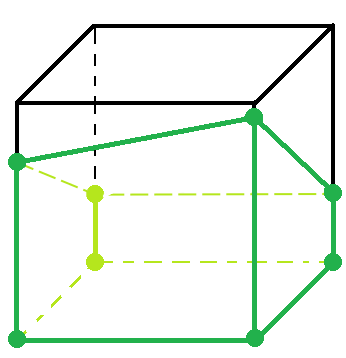
\includegraphics[ width=70mm]{../img/analysis/krychle}

\caption{Příklad nastavení polygonů}
\label{fig:polygons}

\end{figure}

\FloatBarrier

Obrázek \ref{fig:polygons} nám dává náhled nějakého možného uspořádání pěti polygonů v~rámci krychle. Silně vykreslené body představují definiční \textit{body}, jednotlivé čáry pak \textit{hrany} polygonů. Záměrně jsme neudělali polygony pravidelné, abychom demonstrovali, že je možné se libovolně přizpůsobovat tvarům vycházejícím z~polygonální reprezentace daného bloku.


V rámci algoritmu spojování bloků skrz vodivé spojení pak budeme hledat pro daný blok sousedy právě dle těchto definic. Budeme počítat s~tím, že polygony jsou v~rámci jedné roviny v~prostoru, přičemž daná rovina je rovnoběžná s~některou z~rovin mřížky herního světa. V~rámci této práce si algoritmus usnadníme takovým způsobem, že jednotlivé studované polygony rozšíříme na \textit{boxy}, tedy najdeme nejmenší možný kvádr, který je zarovnaný do mřížky definované herním světem (tedy nemá vůči ní žádnou rotaci) a~obsahuje všechny body z~daného polygonu\footnote{Abychom mohli použít standardních metod \TT{FBox::Intersect(...)}, musíme \textit{box} rozšířit o~něco netriviálního (např. $1~cm$) ve směru normály dané roviny.}. Za validní a~vodivé elektrické vedení pak budeme považovat takové dva polygony, které mají neprázdný průnik těchto boxů. Jsme si vědomi faktu, že tato úprava jde proti snahám hry o~vyšší stupeň realismu a~pro některé kombinace bloků dokonce bude porušovat naši definici vodivého spojení, ale v~této fázi nám to stačí a~nebudeme vyžadovat matematicky správné řešení.


\subsection{Objekt elektrické sítě}

Spojování bloků do elektrické sítě nevyžaduje žádnou speciální logiku. V~rámci přidávání bloku do herního světa budeme potřebovat vědět o~sousedních blocích (TODO stromy). Pokud bude vazba se sousedním blokem vyhodnocena jako validní vodivý spoj, může se nově připojený blok připojit ke stávající síti, v~níž je i~daný sousední blok.

Pokud budeme vycházet z~premisy, že každý blok je zapojen právě v~jedné elektrické síti a~všechny bloky v~rámci jedné elektrické sítě jsou mezi sebou vodivě spojeny, tak nutně musíme dojít k~závěru, že při manipulaci s~blokem budeme muset elektrické sítě aktualizovat. Přidáním bloku jsme bychom mohli vodivě propojit dvě či více sítí, při odebírání se nám daná elektrická síť může rozpadnout na více samostatných komponent. Těchto elektrických sítí může vznikat a~zanikat velké množství. Stačí si uvědomit, že k~bloku \nameref{blocks:A1} o~maximální možné velikosti můžeme připojit až 600 bloků, které budou patřit do stejné sítě (pro každou stěnu máme 100 bloků stejného typu a~minimální velikosti, uspořádaných do šachovnicového vzoru). Pokud pak odebereme centrální blok, může nám vzniknout právě až 600 nových elektrických sítí. Navíc, díky počasí se může stát, že bloky budou odebírány ze světa zcela neuspořádaně (na základě náhodně udělovaného poškození). Musíme tedy vymyslet algoritmus, jak pro všechny bloky v~herním světě udržovat správné informace o~jejich síti.

Protože nemůžeme nic předpokládat o~tom, jak se budou bloky v~elektrické síti chovat, musíme při změně (přidání či odebrání) nějakého bloku v~síti provést přepočítání. Nejjednodušší bude varianta na \textit{algoritmus vlny}. Jednotlivé sítě budeme podle potřeby odstraňovat či slévat. Popišme si nyní pravidla, která budeme muset ve hře mít. Jako sousedy budeme chápat bloky dostupné skrze vodivé spojení.

\subsubsection{Přidávání bloku}
Platí, že každý blok přidaný do herního světa si vytvoří svoji vlastní elektrickou síť.
(TODO kontrola enums níže)
\begin{enumerate}
	\item Pokud blok nemá žádné sousedy, nemusí dělat nic (svoji síť už má)
	\item Pokud mají všichni sousedé stejnou síť, blok se k~ní připojí
	\item Pokud mezi sousedy existují alespoň dvě různé elektrické sítě, blok si vytvoří novou elektrickou síť, propojí ji s~ostatními sítěmi a~vyvolá přepočet sítí
\end{enumerate}

\subsubsection{Odebírání bloku}
Platí, že každý odebíraný blok z~herního světa vždy odstraní síť, ve které je připojen, a~pro všechny jeho sousedy jsou vytvořeny nové sítě.

\begin{enumerate}
	\item Pokud blok nemá žádné sousedy, svoji síť ze hry odstraní a~dále nedělá nic
	\item Pokud má blok právě jednoho souseda, odpojí od se od dané sítě
	\item Pokud má alespoň dva sousedy, pro každého vytvoří novou síť a~vyvolá přepočet sítí
\end{enumerate}

\subsection{Udržování konzistence elektrických sítí}

Jak je vidět z~předchozí kapitoly, objektů k~aktualizaci může být velmi mnoho. Nesmíme však dopustit, aby se nám při přepočítávání začala hra zpomalovat či přímo zasekávat\footnote{Tato situace může snadno nastat, protože herní a~renderovací smyčky se na konci svých cyklů synchronizují, aby pro výpočet dalšího framu začínaly stejně.}. Opět máme více možností řešení, jak se k~tomuto problému postavit. 

Jedním z~možných řešení je spuštění výpočtů na samostatném výpočetním vlákně. Zde bohužel narážíme na problém, že výpočty ve vláknech v~\UEu{} nemohou přímo přistupovat k~herním objektům a~tudíž je nutné používat pomocných datových struktur a~výsledky poté zpětně propagovat. Kromě toho také narážíme na problém, kdy v~případě velmi silné bouře kyselých dešťů bude nejspíše často nutné výpočet předčasně ukončit a~spustit znovu.

My navrhujeme následující algoritmus, využívající front požadavků ke zpracování a~omezení výpočetního času. Ještě musíme zmínit, že také využívá toho, že jak elektrická síť, tak každý blok v~ní si nese informaci o~stavu. Ty jsou tři:
\begin{itemize}
	\item Nevalidní
	\item Ve výpočtu
	\item Validní
\end{itemize}
Volba stavů je zřejmá a~vychází z~principů algoritmu vlny. Dalším netriviálním faktem je, že v~algoritmu existuje fronta sítí k~přepočítání, přičemž každá taková má svoji frontu bloků v~síti k~přepočítání. Hlavním krokem algoritmu je pak výběr sítě k~přepočítání a~provedení jednoho kroku přepočtu. Následně, pokud má tato síť stále nějaké bloky k~přepočtu, je zařazena na konec přepočítávací fronty a~tam čeká, dokud nebude opět vyzvednuta. Může se však stát, že jistou posloupností kroků při mazání bude tato síť označena jako nevalidní a~dále se přepočítávat nebude.

Algoritmus bude mít přidělené nějaké maximální kvantum času, řekněme tak, aby při jeho výpočtech hra dosahovala alespoň 30 snímků za sekundu. Tím vcelku jednoduchým a~elegantním způsobem zajistíme přepočty i~pro velice rozsáhlé sítě. Samozřejmě je nutné, aby hra počítala s~tím, že elektrická síť a~bloky v~ní mohou být ve stavu \textit{ve výpočtu} a~tomu přizpůsobovat další funkcionalitu (například nevyužívat zdrojů takovéto sítě, dokud blok není \textit{validní} -- pak je možné využívat pouze dalších validních bloků, tedy těch, které již byly zpracovány algoritmem).

TODO tabulka případů, říct, že tohle bude komponenta

\subsection{Interakce a~označování}
\label{subsec:interaction}

Dalším problémem je interakce s~uživatelem. Abychom věděli, že hráč s~daným blokem chce interagovat, musíme vědět, že:
\begin{itemize}
	\item Je dostatečně blízko bloku
	\item Z~pohledu hráče se dívá na daný blok 
	\item Vyjadřuje fakt, že chce interagovat (např. stiskem klávesy)
\end{itemize}



Nejsnazší způsob, jak zjistit, na jaký herní objekt se hráč dívá, je použití techniky sledování paprsku (\textit{ray tracing}). Díky němu můžeme \uv{z kamery} vyslat virtuální paprsek, který má stejný směr, jako je směr pohledu kamery. Pokud bude hráčův \HUD{} zobrazovat zaměřovací kříž (či použijeme nějaký obdobný mechanismus) a~náš paprsek bude z~pohledu kamery tímto zaměřovačem procházet, hráč může cíleně mířit na herní objekty a~my zároveň budeme mít správnou informaci o~objektu, na který hráč zaměřovačem míří. Tento způsob získávání informace o~objektech v~hráčově zaměřovači je ve hrách běžný a~jeho použití je (pokud je vhodně použito) i~dostatečně rychlé.

Nyní, když už víme, jak můžeme získávat informace o~tom, na který objekt hráč míří, tak tento mechanismus ještě rozšíříme o~další vlastnost. Je zapotřebí si uvědomit, že interakce s~blokem a~umisťování nového herního bloku (případně mazání) jsou prakticky stejné akce. Liší se pouze výsledkem -- reakcí na stisk nějaké klávesy či tlačítka myši. Ale ve všech případech musíme vědět, na jaký blok hráč míří zaměřovačem, u~umisťování navíc potřebujeme znát i~přesný polygon, na který hráč míří. Konkrétní polygon potřebujeme znát z~toho důvodu, že chceme, aby se přidávaný blok \uv{přilepil} k~bloku, na který míříme. Tedy chceme zachovat herní mechaniku, která je v~hrách z~kapitoly \ref{chap:uvod} běžná a~je natolik intuitivní a~rozšířená, že změna této mechaniky by nejspíše nedopadla dobře a~hráči by nebyla kladně přijata.

Pro implementaci nám poslouží metoda \TT{LineTraceSingleByObjectType},\linebreak které předáme správné parametry (především počátek a~konec paprsku a~typy objektů, které paprsek zaznamená) a~ta nám vrátí strukturu, popisující výsledek trasování. Z~něj se můžeme dozvědět, jestli byl nějaký blok v~cestě paprsku. A~pokud ano, můžeme se ptát, zda měl komponentu interakce (potenciálně bychom mohli chtít bloky bez možnosti zaměření a~interakce, jakožto nesmazatelné objekty). Pokud bude i~tato podmínka splněna, můžeme se zajímat o~další vlastnosti kolize paprsku s~blokem a~na základě toho se nějak chovat.

Abychom hráči hraní usnadnili a~zpříjemnili, budeme bloky zvýrazňovat za použití techniky \textit{obrysu} (implementace zvýrazňování bude vycházet z~tutorialu~\citep{ue_outline_tut}). Tato technika je také využívána v~různých hrách napříč různými herními žánry a~proto její implementací nic nezkazíme. Obrys zobrazíme v~případě, kdy hráč nic nestaví a~daný označený blok je použitelný (takže hráč ví, že blok může používat), nebo v~případě, kdy hráč staví (zvýrazníme hranice namířeného objektu). Barvu obrysu můžeme zvolit kupříkladu zelenou pro použitelný blok, žlutou při stavění a~červenou při odebírání bloku. 


\subsection{Umístění ve světě}

Smyslem této komponenty je oddělení implementace bloku jako takového a~implementace herního světa. Skrze tuto komponentu se blok bude moci dotazovat na ostatní bloky v~herním světě, především pak bloky ve svém okolí. To bude důležité například pro elektrickou komponentu, která na základě \uv{sousedství} bude jednotlivé bloky vázat k~sobě do elektrické sítě.








\section{Definice bloků}
\label{sec:db}

Jak bylo řečeno v~analýze v~části \ref{sec:chceme}, potřebujeme u~bloků definovat mj.~následující vlastnosti: \textit{minimální} a~\textit{maximální} velikost, \textit{typ} bloku, možnost \textit{rotace} bloku dle daných os apod. Dále budeme u~bloků potřebovat zaznamenat, že blok má \textit{elektrickou} či \textit{kyslíkovou} komponentu a~definovat omezující vlastnosti této komponenty. Dále požadujeme, abychom mohli snadno modifikovat hodnoty těchto vlastností. Tento požadavek vznášíme z~toho důvodu, aby herní designér mohl rychle a~jednoduše ladit nastavení těchto konstant a~vyvažovat tak celkovou obtížnost hry. Takže nepřipadá v~úvahu, abychom měli tyto konstanty uložené ve zdrojovém kódu, protože jakákoliv úprava by znamenala opětovnou kompilaci hry a~to u~herních projektů často zabere netriviální čas. Pak je ale budeme muset načítat z~nějakého souboru, nebo budou muset být uložené v~nějakém definičním objektu, editovatelným z~Editoru.


\subsection{Textové soubory}
Při načítání definic z~textového souboru máme na výběr z~více možností. V~následujících odstavcích si jednotlivé možnosti popíšeme a~zamyslíme se nad výhodami a~nevýhodami daných přístupů. Jednu výhodu však mají všechny textové přístupy společnou -- snadnou čitelnost i~pro běžného člověka.

\subsubsection{Popis tabulkou}
Uvažme popis bloků v~nějakém tabulkovém formátu, třeba CSV. Pokud\linebreak bychom měli velice málo vlastností bloků, tento přístup by mohl být použitelný. Nicméně s~každým dalším nově přidaným blokem se do množiny všech vlastností mohou zanášet nové vlastnosti. To by znamenalo, že popis ostatních bloků, které danou vlastnost nemají, by musel nutně v~tomto tabulkovém zápisu uvažovat nějakou (byť prázdnou) hodnotu. Zbytečně by nám tak rostl definiční soubor. Další nevýhodou je absence typové bezpečnosti pro uložené hodnoty. 

\subsubsection{Popis samostatným souborem -- XML}
Běžné soubory textového formátu (TXT) není potřeba brát v~potaz. Výsledek je stejný jako při použití XML, ale nemůžeme zde použít definiční soubory pro automatickou kontrolu platnosti hodnot. Navíc bychom museli psát vlastní parser takového textového souboru, přičemž již hotové parsery XML jsou volně k~dispozici a~mohli bychom je snadno použít. Definici herních bloků v~XML využívá i~hra \ME{}. Tyto soubory jsou pak zpracovány herním enginem během načítání hry. Výhodou tohoto přístupu je, kromě snadného vytváření módu do hry, také snadná budoucí rozšiřovatelnost o~nové bloky.

\subsection{Binární zápis}
Binární zápis již není pro běžného člověka tak snadno čitelný, ale to nám nemusí vadit, pokud budeme mít k~dispozici příslušné editační rozhraní. My si totiž můžeme v~\UEu{} připravit třídu, jejíž vlastnosti jsou z~Editoru editovatelné pouze v~rámci nastavování výchozích hodnot. To znamená, že si na straně \CPP{} můžeme vhodným způsobem vytvořit strukturu definičních tříd, které následně použijeme v~Editoru. Na straně \UEu{} pak vytvoříme Blueprint, který bude dědit z~naší hlavní definiční třídy. Posléze můžeme této třídě upravovat výchozí hodnoty a~tímto způsobem tak definovat vlastnosti bloků.

Kromě toho, že tímto přístupem splňujeme požadavek na editovatelnost z~Editoru, získáváme také navíc typovou bezpečnost uložených hodnot. Dále máme možnost (v případě nějakých definičních specialit) vytvořit vlastní editační panely pro dané netriviální vlastnosti definičního souboru. 


\subsection{Definice bloků -- verdikt}

Na základě výše zmíněných poznatků jsme se rozhodli, že budeme bloky definovat v~binárním formátu. V~\CPP{} implementujeme definiční třídu s~vhodnou strukturou a~v~Editoru pak následně vytvoříme Blueprintové assety, ve kterých požadované vlastnosti pro námi požadované bloky nadefinujeme. Získáme tak možnost snadné úpravy požadovaných vlastností v~Editoru a~typovou bezpečnost vyplněných hodnot.